\documentclass[12pt]{amsart}

\usepackage{amsthm}
\usepackage{amssymb}
\usepackage{amsmath}
\usepackage{tikz}
\usetikzlibrary{shapes.geometric,calc}
\usepackage{geometry}
\geometry{a4paper}

\newtheorem{thm}{Theorem}
\newtheorem{prop}{Proposition}
\newtheorem{lem}{Lemma}
\newtheorem{cor}{Corollary}
\newtheorem{rem}{Remark}
\newtheorem{exa}{Example}
\newtheorem{clm}{Claim}

\title{DeMorgan's Laws and Hexagonal Symmetry}
\author{Jason Medcoff}

\begin{document}
	
	\maketitle
	
	\section{DeMorgan's Laws}
	
	\begin{clm}
		For any two sets $A$ and $B$, $(A \cup B)^{\complement} = A^{\complement} \cap B^{\complement}$.
	\end{clm}
	
	\begin{proof}
		
		Let $x \in (A \cup B)^{\complement}$. Then $x \notin A \cup B$. It must be the case that $x \notin A$ and $x \notin B$. Thus, $x \in A^{\complement}$ and $x \in B^{\complement}$, so $x \in A^{\complement} \cap B^{\complement}$. This means that $\forall x \in (A \cup B)^{\complement}$, $x \in A^{\complement} \cap B^{\complement}$.
		By the definition of set inclusion, $(A \cup B)^{\complement} \subset A^{\complement} \cap B^{\complement}$.
		$\newline$
		
		Let $y \in A^{\complement} \cap B^{\complement}$. Then $y \in A^{\complement}$ and $y \in B^{\complement}$. So $y \notin A$ and $y \notin B$. Therefore, $y \notin A \cup B$, so it must be that $y \in (A \cup B)^{\complement}$. Similar to above, it follows that $A^{\complement} \cap B^{\complement} \subset (A \cup B)^{\complement}$.
		$\newline \newline$
		By definition of set equality, $(A \cup B)^{\complement} = A^{\complement} \cap B^{\complement}$.	 		
	\end{proof}
	
	\begin{clm}
		For any two sets A and B, $(A \cap B)^{\complement} = A^{\complement} \cup B^{\complement}$.
	\end{clm}
	
	\begin{proof}
		Let $x \in (A \cap B)^{\complement}$. Then $x \notin A \cap B$. So $x\notin A$ or $x \notin B$. Therefore $x \in A^{\complement}$ or $x \in B^{\complement}$. Thus, $x \in A^{\complement} \cup B^{\complement}$. By the definition of set inclusion, $(A \cap B)^{\complement} \subset A^{\complement} \cup B^{\complement}$.
		$\newline$
		
		Let $y \in A^{\complement} \cup B^{\complement}$. It follows that $y \in A^{\complement}$ or $y \in B^{\complement}$. Then $y \notin A$ or $y \notin B$. So $y \notin A \cap B$, therefore $y \in (A \cap B)^{\complement}$. Similar to above, we find that $A^{\complement} \cup B^{\complement} \subset  (A \cap B)^{\complement}$.
		$\newline$
		By definition of set equality, $(A \cap B)^{\complement} = A^{\complement} \cup B^{\complement}$.
	\end{proof}
	
	
	\section{The Regular Hexagon}
	
    %	A regular hexagon is a six sided polygon such that all angles are equal in measure and all sides have the same length. One can draw a right triangle inside a regular hexagon to determine that the radius of a circumscribed circle is equal to the side length of the hexagon. Thus, a regular hexagon can be constructed with compass and straightedge by making a circle, then using its radius to draw equally spaced points along its circumference, labeled $\mathit{1}, \mathit{2}, \mathit{3}, \mathit{4}, \mathit{5},$ and $\mathit{6}$.
    %	
    %	The regular hexagon as labeled has twelve symmetries: six rotational and six reflectional. Rotating the hexagon counterclockwise by an integer multiple of 60 degrees gives a symmetry, so the six rotational symmetries are 60, 120, 180, 240, 300, and 360 degrees. 
    %	
    %	The reflectional symmetries can be obtained by defining the axes of symmetry on the polygon. Three of the axes are constructed by connecting opposite vertices. The remaining three are found by bisecting each side of the hexagon. Thus, the six reflectional symmetries are given by the line segments $\overline{\mathit{14}}, \overline{\mathit{25}}, \overline{\mathit{36}}, \overline{AD}, \overline{BE},$ and $\overline{CF}$.
	
	A regular hexagon is a six sided convex polygon such that all interior angles are equal in measure and all sides have the same length. Consider a regular hexagon inscribed in a circle with center $O$ and radius $r$. Label the vertices of the hexagon $\mathit{1}$, $\mathit{2}$, $\mathit{3}$, $\mathit{4}$, $\mathit{5}$, and $\mathit{6}$.
	
	\begin{center}

		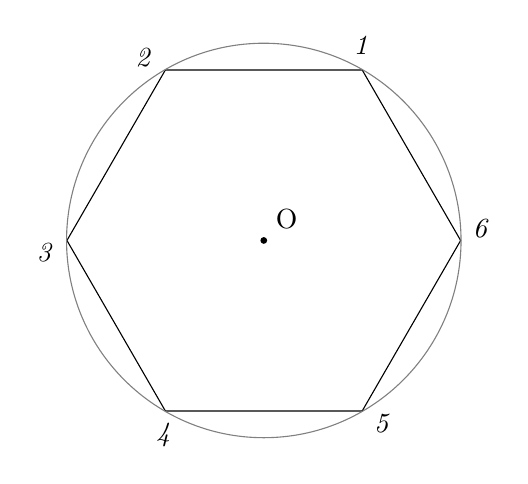
\begin{tikzpicture}
		\node[regular polygon,regular polygon sides=6,draw,minimum height=5cm] (a) at (0,0) {};
		\draw[gray] let \p1=($(a.corner 1)-(a.center)$), \n1={veclen(\x1,\y1)} in circle (\n1);
		\filldraw (0,0) circle[radius=1.0pt];
		\node[above right, outer sep=1pt] (0,0) {O};
		\foreach \x[count=\xi] in {$\mathit{1}$, $\mathit{2}$, $\mathit{3}$, $\mathit{4}$, $\mathit{5}$, $\mathit{6}$}{
		\node (a-\xi) at ([shift={({90+(\xi-1)*360/6}:3mm)}]a.corner \xi) {\x};
		}
		\end{tikzpicture}
		
	\end{center}
	
	
	
	
	
	
	
	
	
	
	
	
	\begin{clm}
		  The hexagon has side length $r$.
	\end{clm}
	
	\begin{proof}
		Consider the triangle $O\mathit{12}$. We know this is an isosceles triangle because $\overline{O\mathit{1}}$ and $\overline{O\mathit{2}}$ are both radii of the circle. Since each interior angle of the regular hexagon is 120 degrees, we know $\angle O\mathit{12} = \angle O\mathit{21} = 60^{\circ}$. Therefore, because the sum of the interior angles of a triangle is 180 degrees, $\angle \mathit{1} O \mathit{2} = 180 - 2(60) = 60$. Thus, $O\mathit{12}$ is an equilateral triangle, and $\overline{O\mathit{1}} = \overline{O\mathit{2}} = \overline{\mathit{12}}$. But $\overline{\mathit{12}}$ is the side of the hexagon, and $\overline{O\mathit{1}}$ is a radius $r$. So, the hexagon has side length $r$.
	\end{proof}
	
	The regular hexagon has twelve symmetries. Six are rotational, and the remaining six are reflectional. Let the pre-image be defined as the polygon before it is transformed, and the image is the polygon after it is transformed. With each transformation, a vertex will be mapped to the position of another. Using this notation we can write the reflectional symmetries.
	
	$\newline$
	
	\begin{tabular}{ccc}
	
	\begin{tabular}{c | c}
		pre-image & image \\
		\hline
		$\mathit{1}$ & $\mathit{2}$ \\
		$\mathit{2}$ & $\mathit{3}$ \\
		$\mathit{3}$ & $\mathit{4}$ \\
		$\mathit{4}$ & $\mathit{5}$ \\
		$\mathit{5}$ & $\mathit{6}$ \\
		$\mathit{6}$ & $\mathit{1}$	
	\end{tabular}
	
	&
	
	\begin{tabular}{c | c}
		pre-image & image \\
		\hline
		$\mathit{1}$ & $\mathit{3}$ \\
		$\mathit{2}$ & $\mathit{4}$ \\
		$\mathit{3}$ & $\mathit{5}$ \\
		$\mathit{4}$ & $\mathit{6}$ \\
		$\mathit{5}$ & $\mathit{1}$ \\
		$\mathit{6}$ & $\mathit{2}$	
	\end{tabular}

    &
    
    \begin{tabular}{c | c}
    	pre-image & image \\
    	\hline
    	$\mathit{1}$ & $\mathit{4}$ \\
    	$\mathit{2}$ & $\mathit{5}$ \\
    	$\mathit{3}$ & $\mathit{6}$ \\
    	$\mathit{4}$ & $\mathit{1}$ \\
    	$\mathit{5}$ & $\mathit{2}$ \\
    	$\mathit{6}$ & $\mathit{3}$	
    \end{tabular}
	
	\end{tabular}
	
	$\newline$

\begin{tabular}{ccc}
	
	\begin{tabular}{c | c}
		pre-image & image \\
		\hline
		$\mathit{1}$ & $\mathit{5}$ \\
		$\mathit{2}$ & $\mathit{6}$ \\
		$\mathit{3}$ & $\mathit{1}$ \\
		$\mathit{4}$ & $\mathit{2}$ \\
		$\mathit{5}$ & $\mathit{3}$ \\
		$\mathit{6}$ & $\mathit{4}$	
	\end{tabular}
	
	&
	
	\begin{tabular}{c | c}
		pre-image & image \\
		\hline
		$\mathit{1}$ & $\mathit{6}$ \\
		$\mathit{2}$ & $\mathit{1}$ \\
		$\mathit{3}$ & $\mathit{2}$ \\
		$\mathit{4}$ & $\mathit{3}$ \\
		$\mathit{5}$ & $\mathit{4}$ \\
		$\mathit{6}$ & $\mathit{5}$	
	\end{tabular}
	
	&
	
	\begin{tabular}{c | c}
		pre-image & image \\
		\hline
		$\mathit{1}$ & $\mathit{1}$ \\
		$\mathit{2}$ & $\mathit{2}$ \\
		$\mathit{3}$ & $\mathit{3}$ \\
		$\mathit{4}$ & $\mathit{4}$ \\
		$\mathit{5}$ & $\mathit{5}$ \\
		$\mathit{6}$ & $\mathit{6}$	
	\end{tabular}
	
\end{tabular}

	$\newline$
	
	An observation here is that every rotation shown is a multiple of 60 degrees, with the 360 degree rotation being the identity of the transformation.
	
	In a similar way, the reflectional symmetries can be shown. 
	
    $\newline$
	
	\begin{tabular}{ccc}
		
		\begin{tabular}{c | c}
			pre-image & image \\
			\hline
			$\mathit{1}$ & $\mathit{6}$ \\
			$\mathit{2}$ & $\mathit{5}$ \\
			$\mathit{3}$ & $\mathit{4}$ \\
			$\mathit{4}$ & $\mathit{3}$ \\
			$\mathit{5}$ & $\mathit{2}$ \\
			$\mathit{6}$ & $\mathit{1}$	
		\end{tabular}
		
		&
		
		\begin{tabular}{c | c}
			pre-image & image \\
			\hline
			$\mathit{1}$ & $\mathit{5}$ \\
			$\mathit{2}$ & $\mathit{4}$ \\
			$\mathit{3}$ & $\mathit{3}$ \\
			$\mathit{4}$ & $\mathit{2}$ \\
			$\mathit{5}$ & $\mathit{1}$ \\
			$\mathit{6}$ & $\mathit{6}$	
		\end{tabular}
		
		&
		
		\begin{tabular}{c | c}
			pre-image & image \\
			\hline
			$\mathit{1}$ & $\mathit{4}$ \\
			$\mathit{2}$ & $\mathit{3}$ \\
			$\mathit{3}$ & $\mathit{2}$ \\
			$\mathit{4}$ & $\mathit{1}$ \\
			$\mathit{5}$ & $\mathit{6}$ \\
			$\mathit{6}$ & $\mathit{5}$	
		\end{tabular}
		
	\end{tabular}
	
	$\newline$
	
	\begin{tabular}{ccc}
		
		\begin{tabular}{c | c}
			pre-image & image \\
			\hline
			$\mathit{1}$ & $\mathit{3}$ \\
			$\mathit{2}$ & $\mathit{2}$ \\
			$\mathit{3}$ & $\mathit{1}$ \\
			$\mathit{4}$ & $\mathit{6}$ \\
			$\mathit{5}$ & $\mathit{5}$ \\
			$\mathit{6}$ & $\mathit{4}$	
		\end{tabular}
		
		&
		
		\begin{tabular}{c | c}
			pre-image & image \\
			\hline
			$\mathit{1}$ & $\mathit{2}$ \\
			$\mathit{2}$ & $\mathit{1}$ \\
			$\mathit{3}$ & $\mathit{6}$ \\
			$\mathit{4}$ & $\mathit{5}$ \\
			$\mathit{5}$ & $\mathit{4}$ \\
			$\mathit{6}$ & $\mathit{3}$	
		\end{tabular}
		
		&
		
		\begin{tabular}{c | c}
			pre-image & image \\
			\hline
			$\mathit{1}$ & $\mathit{1}$ \\
			$\mathit{2}$ & $\mathit{6}$ \\
			$\mathit{3}$ & $\mathit{5}$ \\
			$\mathit{4}$ & $\mathit{4}$ \\
			$\mathit{5}$ & $\mathit{3}$ \\
			$\mathit{6}$ & $\mathit{2}$	
		\end{tabular}
		
	\end{tabular}

    $\newline$
    
    These symmetries are obtained by first reflecting the hexagon, then rotating it as above.
	
	
\end{document}